\documentclass[11pt,a4paper]{article}
\usepackage{termpaper}
\usepackage[utf8]{inputenc}
\usepackage{tabularx,lipsum,environ,amsmath,amssymb,amsthm}
\usepackage{todonotes}
\usepackage{enumerate}

\makeatletter
\newcommand{\problemtitle}[1]{\gdef\@problemtitle{#1}}% Store problem title
\newcommand{\probleminput}[1]{\gdef\@probleminput{#1}}% Store problem input
\newcommand{\problemquestion}[1]{\gdef\@problemquestion{#1}}% Store problem question
\NewEnviron{csproblem}{
  \problemtitle{}\probleminput{}\problemquestion{}% Default input is empty
  \BODY% Parse input
  \par\addvspace{.5\baselineskip}
  \noindent
  \begin{tabularx}{\textwidth}{@{\hspace{\parindent}} l X c}
    \multicolumn{2}{@{\hspace{\parindent}}l}{\textsc{\@problemtitle}} \\% Title
    \textbf{Input:} & \@probleminput \\% Input
    \textbf{Question:} & \@problemquestion% Question
  \end{tabularx}
  \par\addvspace{.5\baselineskip}
}
\makeatother

\makeatletter
\newcommand{\problemparam}[1]{\gdef\@problemparam{#1}}% Store problem input
\NewEnviron{csproblemparam}{
  \problemtitle{}\probleminput{}\problemparam{}\problemquestion{}% Default input is empty
  \BODY% Parse input
  \par\addvspace{.5\baselineskip}
  \noindent
  \begin{tabularx}{\textwidth}{@{\hspace{\parindent}} l X c}
    \multicolumn{2}{@{\hspace{\parindent}}l}{\textsc{\@problemtitle}} \\% Title
    \textbf{Input:} & \@probleminput \\% Input
    \textbf{Parameter:} & \@problemparam \\% Param
    \textbf{Question:} & \@problemquestion% Question
  \end{tabularx}
  \par\addvspace{.5\baselineskip}
}
\makeatother

\theoremstyle{definition}
\newtheorem{definition}{Definition}[section]

\theoremstyle{proposition}
\newtheorem{proposition}{Proposition}[section]

%opening
\title{Fixed Parameter Tractability of SAT through Backdoors}
\author{
 \authorname{Rupert Ettrich} \\
 \studentnumber{01129393} \\
 \curriculum{066 931 Logic and Computation} \\
 \email{rupert.ettrich@gmail.com}
}

\begin{document}

\maketitle

\begin{abstract}
Lorem ipsum dolor sit amet, consectetur adipisicing elit, sed do eiusmod tempor incididunt ut labore et dolore magna aliqua. Ut enim ad minim veniam, quis nostrud exercitation ullamco laboris nisi ut aliquip ex ea commodo consequat. Duis aute irure dolor in reprehenderit in voluptate velit esse cillum dolore eu fugiat nulla pariatur. Excepteur sint occaecat cupidatat non proident, sunt in culpa qui officia deserunt mollit anim id est laborum. \todo{Write abstract}
\end{abstract}

\section{Introduction}

The Satisfiability Problem (SAT) is a fundamental problem in logic and computer science. Given a formula $F$ in propositional logic, the task is to determine whether there exists some assignment of variables in $F$ to the truth values $\{0,1\}$ such that the formula is evaluated to $1$. The simplicity of its definition makes SAT a very powerful modeling tool for many different problems related to software and hardware planning and design. For many such problems it is easier to express it as a propositional logic formula where a satisfying variable assignment can be transformed into a solution of the original problem, and use a SAT-solver on the instance than to develop a problem-specific algorithm. 

The famous Cook-Levin Theorem \cite{Cook71, Levin73} states that SAT belongs to the class of NP-Complete problems. This means that, although it is easy to verify a solution, the existence of an efficient polynomial time algorithm to solve any given instance seems highly unlikely. However, despite the theoretical worst-case complexity of the problem, many large real-world SAT instances can be solved rather efficiently by modern SAT-solvers. This gap between theoretical and practical results lead to research on the structural properties of SAT-instances that can be exploited in order to explain this phenomenon. 

The framework of Parameterized Complexity was introduced by Downey and Fellows \cite{downeyFellows} in order provide tools for a more fine-grained analysis of computationally hard problems. This framework allows to consider the runtime of a problem given some fixed parameter. Depending on the chosen parameter, the runtime can differ drastly, which leads to the study of fixed-parameter tractable parameters. In the context of SAT this leads to two (not necessarily exclusive) approaches when studying its parameterized complexity: Structural Decomposition and Backdoors. While the former is comprised of approaches to find and exploit structural properties of the whole input formula, the latter is about finding a small subset of variables whose assignment leads into a tractable class of SAT-instances. In this seminar paper we will focus on showing fixed-parameter tractability results that can be achieved by the latter approach, Backdoors. 

Section \ref{sec:preliminaries} contains information about the necessary preliminaries and notation that is used in this work. Section \ref{sec:boundedbackdoors} gives a general overview of fixed-parameter tractability and intractability results regarding Backdoors of bounded size. These results are based on a survey of Gaspers and Szeider \cite{Gaspers2012}. Section \ref{sec:unboundedbackdoors} contains recent contributions to research regarding Backdoors of unbounded size. Finally, section \ref{sec:conclusions} summarizes the results shown in this seminar paper and offers some concluding remarks. 

\section{Preliminaries}
\label{sec:preliminaries}
This section contains definitions of the general concepts used in context with Backdoors in SAT. We conform to the notation and definition for SAT, Base Classes, and Backdoor Sets used by Gaspers and Szeider \cite{Gaspers2012} and give a brief introduction on fixed-parameter tractability as defined by Cygan et al \cite{Cygan2015}. Note that section \ref{sec:relatedwork} contains additional definitions and notation specific to the presented material. 
\subsection{The Satisfiability Problem}
The Satisfiability Problem, Boolean Satisfiability Problem, or SAT is a fundamental problem in computer science with many applications in software and hardware planning and scheduling, since many problems can be modeled as SAT-instances and solved by SAT-solvers. It is an NP-Complete decision problem that can be defined as follows: 
\begin{csproblem}
\problemtitle{SAT}
\probleminput{A propositional logic formula $F$ in conjunctive normal form (CNF) over propositional variables $X = \{x_1, x_2, ... , x_n\}$}
\problemquestion{Is there a truth assignment $\tau: X \to \{0,1\}$ (or $\tau \in 2^X$) such that $F[\tau]$ evaluates to $1$?}
\end{csproblem}

We use the following notation: A literal is a propositional variable $x$ or $x^1$ (positive literal) or a negated variable $\overline{x}$ or $x^0$ (negative literal). A clause is a finite set of literals that does not contain two complementary literals (e.g. $x$ and $\overline{x}$). A SAT-instance is comprised of a propositional logic formula $F$ in conjunctive normal form (CNF), which is a set of clauses, where the literals inside each clause are only connected by the binary operator "logical or" ($\lor$) and the clauses are connected only by the binary operator "logical and" ($\land$). We denote as $k-CNF$ the set of propositional logic formulae in conjunctive normal form that contain at most $k$ literals in each clause. When describing a formula $F$, we use the following equivalent notations: $F = \{ \{x_1, \overline{x_2}\}, \{x_3\} \} = (x_1 \lor \overline{x_2}) \land x_3$. We call a clause $C$ containing only positive literals a \textit{postivie clause}, and a clause containing only negative literals a $\textit{negative clause}$. 

If not stated otherwise, we use $F$ to describe a formula, and $C \in F$ to describe a clause. We denote as $var(F)$ the set of all variables that appear in a formula $F$ as a positive or negative literal. Similarly, we denote as $var(C)$ the set of variables that appear in a clause $C$ as a positive or negative literal. Furthermore, we denote as $n = |var(F)|$ the number of variables and as $m = |\{C \colon C \in F \}|$ the number of clauses in a formula.  

A truth assignment $\tau: X \to \{0,1\}$ is a function that maps the variables in $X \subseteq var(F)$ to the truth values $\{0,1\}$ and we denote as $2^X$ the set of all truth assignments over $X$. For $\tau \in 2^X$ let $\text{true}(\tau) = \{x^{\tau(x)} \colon x \in X\}$ and $\text{false}(\tau) = \{x^{1-\tau(x)} \colon x \in X\}$ be the set of of literals set by $\tau$ to 1 and 0 respectively. We then define $F[\tau] = \{ C \setminus \text{false}(\tau) \colon C \in F, C \cap \text{true}(\tau) = \emptyset \}$. Informally, $F[\tau]$ is the set of clauses that remain after we removing all clauses containing at least one literal that is evaluated to 1 by $\tau$, and removing all literals that are evaluated to 0 by $\tau$ from these remaining clauses. A CNF-formula $F$ is \textit{satisfiable} if there is some $\tau \in 2^{var(F)}$ such that $F[\tau] = \emptyset$, so each clause $C \in F$ contains at least one literal that evaluates to 1 under $\tau$. If there exists no such $\tau \in 2^var(F)$, the formula is \textit{unsatisfiable}. SAT then becomes the problem of deciding whether a CNF-formula $F$ is satisfiable. 

The primal graph of $F$ is a graph whose vertex set consists of exactly of $var(F)$ and two vertices are joined by an edge if the occur together in a clause in $F$. The positive primal graph is defined similarly, but there are only edges between variables that occur together as a positive literal in a clause. The negative primal graph is defined analogously. The incidence graph of $F$ is a bipartite graph whose vertex set is $V_1 \cup V_2$, where $V_1$ contains a vertex for each variable and $V_2$ contains a vertex for each clause. Edges are introduced between two vertices if the variable of the corresponding vertex in $V_1$ appears in the clause of the corresponding vertex of $V_2$. 

We conclude these definitions with a small example. Let $F = (x_1 \lor x_2) \land (\overline{x_3} \lor x_5) \land \overline{x_5}, X_1 = \{x_1, x_5\}$, $\tau_1 \in 2^{X_1}$ s.t. $\tau_1[x_1] = 0, \tau_1[x_5] = 1$. Then $F[\tau_1] = \{\{x_2\}, \{\}\}$ and thus $F[\tau_1]$ is unsatisfiable, as it contains an empty clause. However, for $X_2 = \{x_1, x_3, x_5\}, \tau_2 \in X_2$ s.t. $\tau_2[x_1] = 1, \tau_2[x_3] = 0, \tau[x_5] = 0$ it can easily be seen that $F[\tau_2] = \emptyset$, as each clause is satisfied and therefore $F$ is satisfiable and $\tau_2$ is a satisfying variable assignment. \\


\subsection{Fixed Parameter Tractability}
The framework of Parameterized Complexity is the result of the work of Downey and Fellows \cite{downeyFellows}. In this section we list the definitions of a parameterized problem, fixed-parameter tractability, and W-hardness as defined by Cygan et al. \cite{Cygan2015}.
\begin{definition}[{\cite[Chapter 1, p.12]{Cygan2015}}]
A \textit{parameterized problem} is a language $L \subseteq \Sigma^* \times \mathbb{N}$, where $\Sigma$ is a fixed, finite alphabet. For an instance $(x,k) \in \Sigma^*$, $k$ is called the \textit{parameter}.
\end{definition}
In the context of SAT, this definition corresponds to a pair $(F, k)$, which is a CNF-formula $F$ and some parameter $k$, that is a positive integer that denotes some structural property of the formula, e.g. the treewidth of the primal graph of $F$. 
\begin{definition}[{\cite[Chapter 1, p.13]{Cygan2015}}]
A parameterized problem $L \subseteq \Sigma^* \times \mathbb{N}$ is called \textit{fixed-parameter tractable} (FPT) if there exists an algorithm $\mathcal{A}$ (called a \textit{fixed-parameter algorithm}), a computable function $f : \mathbb{N} \to \mathbb{N}$, and a constant $c$ such that, given $(x,k) \in \Sigma^* \times \mathbb{N}$, the algorithm $\mathcal{A}$ correctly decides whether $(x,k) \in L$ in time bounded by $f(k) \cdot |(x,k)|^c$. The complexity class containing all fixed-parameter tractable problems is called FPT. 
\end{definition}
Intuitively, fixed-parameter tractability can be used as a tool to investigate the complexity of NP-Hard problems in more detail. If an NP-Complete problem is FPT, it means that the combinatorial explosion in the runtime that is expected by NP-Complete problems is restricted to the parameter $k$. Therefore, by fixing the parameter $k$ to a constant value, we obtain a runtime that is polynomial in the size of the input. For SAT, there are many such parameters, e.g. the treewidth of the primal graph of a CNF-formula $F$, or the size $k$ of a strong backdoor set into a tractable class of formulas. However determining the value of the parameter $k$ might be a NP-Complete problem itself (like determining the treewidth of a formula $F$). Furthermore, the selection of the parameter $k$ matters, as some parameters lead to FPT-results, while others do not. This is because there are problems which are assumed to not be FPT. The theory of W[$i$]-hardness, for some $i \geq 1$, can be utilized to show that a problem is most likely not FPT \cite[Chapter 13]{Cygan2015}. This is done by finding a parameterized reduction, that is, a reduction in FPT time, from a W[$i$]-hard problem to the problem for which fixed-parameter intractability is to be shown. 

\subsection{Base Classes}
Backdoors are defined with respect to base classes, which are classes of propositional formulas that can be solved and recognized efficiently. More precisely, a base class $\mathcal{C}$ is defined the following way:
\begin{definition}[{\cite[p.289]{Gaspers2012}}]
\label{def:baseclass}
From a base class we require the following properties: 
\begin{itemize}
\item[(i)] $\mathcal{C}$ can be recognized in polynomial time.
\item[(ii)] The satisfiability of formulas in $\mathcal{C}$ can be decided in polynomial time.
\item[(iii)] $\mathcal{C}$ is closed under isomorphisms (i.e., if two fromulas differ only in the names of their variables, then either both or none belong to $\mathcal{C}$). 
\end{itemize}
\end{definition}
A base class is \textit{clause-induced} if it is closed under subsets, so $F \in \mathcal{C}$ implies $F' \in \mathcal{C}$ for each $F' \subseteq F$, and a base class is \textit{clause-defined} if and only if $\{C\} \in \mathcal{C}$ holds for each clause $C \in F$.
 
What follows is a list of the base classes relevant to this seminar paper, but note that this list is by no means complete. There are many different base classes, but listing results for all of them would be outside of the scope of this seminar paper. We will start with Schaefer's 5 base classes as defined by Gaspers and Szeider \cite[p.290f]{Gaspers2012}:
\begin{enumerate}
\item Horn-formulas: CNF formulas where each clause contains at most one positive literal. 
\item Anti-Horn-formulas: CNF formulas where each clause contains at most one negative literal. 
\item 2-CNF formulas: CNF formulas where each clause contains at most 2 literals
\item 0-valid formulas: CNF formulas where each clause contains at least one negative literal. 0-valid formulas can be recognized easily in time linear in 
\item 1-valid formulas: CNF formulas where each clause contains at least one positive literal. 
\end{enumerate}
As all of these base classes are clause-defined, they can also be recognized in time linear in $m \cdot n$, by checking for each clause whether it is contained in the corresponding base class. Note that for 2-CNF formulas the factor $n$ can be omitted, since clauses can only contain 2 literals at most. Thus, property (i) of definition \ref{def:baseclass} is satisfied. The satisfiability of Horn-formulas and Anti-Horn-formulas can be decided in linear time \cite{HornSAT}, and also the satisfiability of 2-CNF formulas can be decided in linear time $\cite{2SAT}$. For 0-valid formulas deciding the satisfiability is even simpler, as there exists a trivial satisfying assignment for each 0-valid formula which assigns 0 to all variables. Similarly, 1-valid formulas have a trivial satisfying assignment by setting all variables to 1. As the satisfiability of all of Schaefer's base classes can be decided in polynomial time, we conclude that property (ii) of definition \ref{def:baseclass} is also satisfied. 

\todo{Maybe property 3? Subsolver base classes? Base classes for Strong recursive backdoors}

\subsection{Backdoor Sets}
The term \textit{backdoor} was introduced and coined by Williams et al.\cite{typicalCaseComplexity}, where the authors define backdoors and strong backdoors for constraint satisfaction problems, which can be seen as a generalization of SAT. In their work, backdoors are defined with respect to subsolvers, whose definition is similar to base classes. They introduce and use the concept of backdoors to explain the performance of SAT-solvers on large instances with small backdoors, and show empirical evidence for the existence of backdoors in real-world instances. For example, they show an instance with 6783 variables and 437431 clauses that contains a backdoor of only 12 variables. Furthermore, they introduce 3 different algorithms to detect and compute such backdoors, and show that adding randomization increases performance, which serves as an explanation to the observation that many SAT-solvers profit from restarts combined with randomization. 

For backdoors and backdoor sets we conform to the definitions of Gaspers and Szeider \cite{Gaspers2012}. A $\mathcal{C}$-backdoor set is a set is a subset of variables of a CNF-formula $F$ whose assignment leads into a tractable base class $\mathcal{C}$. 
\begin{definition}[{\cite[p.289f]{Gaspers2012}}]
A \textit{strong $\mathcal{C}$-backdoor set} of a CNF-formula $F$ is a set $B$ of variables such that $F[\tau] \in \mathcal{C}$ for each $\tau \in 2^B$. 
\end{definition}
By this definition we can see that, given a strong $\mathcal{C}$-backdoor set of size $k$, we can reduce the satisfiability of $F$ to the satisfiability of $2^k$ formulas in $\mathcal{C}$ and obtain a trivial FPT-algorithm by deciding the satisfiability for all resulting formulas in order to find a satisfying assignment. This can be done in time $2^k \cdot p(F)$, where $p(F)$ denotes some polynomial which is defined by the base class $\mathcal{C}$ and depends only on the input formula $F$. 
\begin{definition}[{\cite[p.289f]{Gaspers2012}}]
A \textit{weak $\mathcal{C}$-backdoor set} of a CNF-formula $F$ is a set $B$ of variables such that $F[\tau]$ is satisfiable and $F[\tau] \in \mathcal{C}$ for some $\tau \in 2^B$. 
\end{definition}
Here we note that a computing a weak $\mathcal{C}$-backdoor already decides $F$, and a satisfying assignment can be obtained in FPT-time by testing for all $2^k$ possible assignments whether the resulting formula is in $\mathcal{C}$ and satisfiable.  
\begin{definition}[{\cite[p.289f]{Gaspers2012}}]
A \textit{deletion $\mathcal{C}$-backdoor set} of a CNF-formula $F$ is a set $B$ of variables such that $F - B \in \mathcal{C}$, where $F - B = \{C \setminus \{x^0, x^1 \colon x \in B\} \colon C \in F \}$. 
\end{definition}
If a class $\mathcal{C}$ is clause-induced, then every deletion $\mathcal{C}$-backdoor set is also a strong backdoor set. This follows from the observation that $F[\tau] \subseteq F - B$ for each $\tau \in 2^B$, because each variable in $B$ can be either set to true or false. If a truth assignment $\tau$ of variables in $B$ sets all literals in a clause to 0, the resulting clause is equivalent to the corresponding clause in the deletion $\mathcal{C}$-backdoor set. If $\tau$ sets a literal in a clause to 1, then the clause disappears in $F[\tau]$. Thus, the previous observation holds. 

Furthermore, if a class $\mathcal{C}$ is closed under unions, then strong backdoor sets and deletion backdoor sets conincide, as $\bigcup_{\tau \in 2^B} F[\tau] = F - B$. This observation can easily be verified by inspecting any clause in $F$ with $var(C) \cap B \neq \emptyset$. Since $C$ contains no complementary literals, we can find a truth assignment such that the literal for each variable in $var(C) \cap B$ is set to 0. The clause that results from this truth assignment is then equivalent to the clause that results from deleting the variables in $B$. 

As shown above, for some base classes strong backdoor sets and deletion backdoor sets conincide. Therefore it is sometimes simpler to consider only strong backdoor sets or only deletion backdoor sets for some base classes. This holds for example for Schaefer's base classes, as all of them are clause-induced and closed under unions. 
\section{Results for Backdoors of bounded size}
\label{sec:boundedbackdoors}

In this section we will give an overview of FPT results and intractability results for the detection of strong and weak backdoor sets of size $k$. The results in this section were presented and compiled in a survey of Gaspers and Szeider \cite{Gaspers2012}. 

\subsection{Strong Backdoor Set Detection}
\label{sec:strongdetection}
For each base class we can define the corresponding strong $\mathcal{C}$-backdoor set detection problem as the following parameterized decision problem: 
\begin{csproblemparam}
        \problemtitle{Strong $\mathcal{C}$-Backdoor Set Detection}
        \probleminput{A CNF formula $F$ and an integer $k \geq 0$}
        \problemparam{The integer $k$}
        \problemquestion{Does $F$ have a strong $\mathcal{C}$-backdoor set of size at most $k$?}
\end{csproblemparam}
In addition to the decision, whether $F$ has a strong $\mathcal{C}$-backdoor, we are primarily interested in functional approaches that also compute such a backdoor set if it exists. If the corresponding strong backdoor set detection problem is FPT, and SAT is FPT parameterized by the size of a strong $\mathcal{C}$-backdoor set, then any SAT instance can be solved in FPT time by first computing a strong $\mathcal{C}$-backdoor and then solving the instance by using this backdoor set. 

As we have shown already, SAT is FPT parameterized by the size of a strong backdoor set into each of Schaefer's base classes. We will now show the results for the corresponding strong backdoor set detection problems.
\begin{proposition}[{\cite[Proposition 5, p.297]{Gaspers2012}}, {\cite{Nishimura}}]
\textsc{Strong $\mathcal{C}$-Backdoor Set Detection} is fixed-parameter tractable for every base class $\mathcal{C} \in \text{Schaefer}$. For $\mathcal{C} \in \{0-\textsc{Val}, 1-\textsc{Val}\}$, the problem is even solvable in polynomial time. 
\end{proposition}

For a CNF-formula $F$ it can easily be seen that the set of deletion Horn-backdoor set corresponds exactly to the set of vertex covers of the positive primal graph of $F$, therefore the fixed-parameter tractability of \textsc{Vertex Cover} can be utilized to find a strong Horn-backdoor set in FPT time. As we observed before, strong backdoor sets and deletion backdoor sets coincide for Schaefer's base classes. Thus, fixed-parameter tractability of strong Horn-backdoor set detection follows. Strong Anti-Horn-backdoor set detection can be solved symmetrically by finding vertex covers of the negative primal graph of $F$.  

For Strong 2-CNF-backdoor set detection the authors present a reduction to \textsc{3-Hitting Set}, which is another fixed-parameter tractable problem. They define a hypergraph whose vertex set consist of exactly the variables in $F$. For each clause $C$ containing more than 2 literals a hyperedge is introduced for each distinct subset of exactly 3 variables $x_1,x_2,x_3$, such that $x_1,x_2,x_3 \in var(C)$. By this reduction we obtain an instance of \textsc{3-Hitting Set} where each hitting set corresponds to a deletion 2-CNF-backdoor set and thus a strong 2-CNF-backdoor set. An example for this reduction can be seen in figure \ref{fig:2cnf-to-3hittingset}

For 0-valid and 1-valid formulas, the authors state that the smallest strong 0-valid-backdoor set of $F$ is exactly the union of $var(C)$ for all positive clauses in $F$, whereas the smallest strong 1-valid-backdoor set of $F$ is the union of $var(C)$ for all negative clauses in $F$. 

\begin{figure}
        \centering
        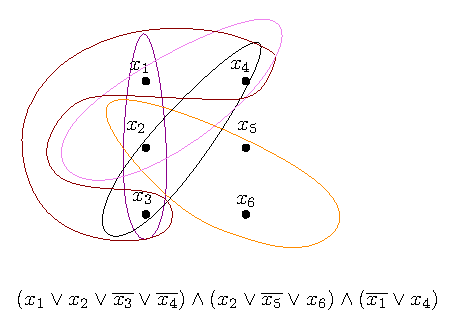
\includegraphics[width=0.5\textwidth]{figures/hitting_set.eps}
        \label{fig:2cnf-to-3hittingset}
	\caption{For each clause $C$ containing at least 3 variables a hypedge for each 3-element subset of $var(C)$ is introduced. In this figure, $\{x_1, x_2\}$ hits all hyperedges and is both a 3-hitting set and a strong 2-CNF-backdoor set.}
\end{figure}


\subsection{Weak Backdoor Set Detection}

Analogously to section \ref{sec:strongdetection} we the decision problem for weak $\mathcal{C}$-backdoor set detection can be defined as follows:
\begin{csproblemparam}
    \problemtitle{Weak $\mathcal{C}$-Backdoor Set Detection}
    \probleminput{A CNF formula $F$ and an integer $k \geq 0$}
    \problemparam{The integer $k$}
    \problemquestion{Does $F$ have a weak $\mathcal{C}$-backdoor set of size at most $k$?}
\end{csproblemparam}
\begin{proposition}[{\cite[Proposition 1, p.293f]{Gaspers2012}}]
\textsc{Weak $\mathcal{C}$-Backdoor Set Detection} is \text{W[2]}-hard for all base classes $\mathcal{C}\in \text{Schaefer}$.
\end{proposition} 
For weak $\mathcal{C}$-backdoor set detection, Gaspers and Szeider show that the problem is W[2]-hard for Schaefer's base classes and thus most likely fixed-parameter intractable. This is done by providing parameterized reduction from \textsc{Hitting-Set}, which is a W[2]-hard problem. However, the proof is rather long and intricate, therefore we will omit it and refer to the paper by Gaspers and Szeider.

However, if there are some restrictions on the input formulas, FPT results can be obtained for weak backdoor set detection. More precisely, Gaspers and Szeider show that weak $\mathcal{C}$-backdoor set detection is FPT if $\mathcal{C}$ is clause induced and the input formula is in $d$-CNF for some constant $d$. 
\begin{proposition}[{\cite[Proposition 2, p.294f]{Gaspers2012}}]
For every clause-defined class $\mathcal{C}$, \textsc{Weak $\mathcal{C}$-Backdoor Set Detection} is fixed-parameter tractable for input formulas in 3-CNF.
\end{proposition}
The proof follows from a bounded search tree argument. Given a formula $F \notin \mathcal{C}$, there must be a clause in $C \in F$ such that $\{C\} \notin \mathcal{C}$. A weak $\mathcal{C}$-backdoor set of $F$ must contain at least one variable of $C$. Since there are at most 3 variables in each clause, the branching of the search tree is limited by $3 \cdot 2$, since we can assign to each variable in $C$ either true or false, and if there exists a weak $\mathcal{C}$-backdoor set of size $k$, then one of these assignments must lead to a satisfying assignment. Since we are looking for a backdoor set of size $k$, the depth of the search tree is bounded by $k$. Finally, for each leaf $t$ of the tree we can obtain a truth assignment $\tau_t$ over $k$ variables. Since the number of leaves in the tree is bounded by $O(6^k)$, we can check for each leaf $t$ and each formula $F[\tau_t]$, whether $F[\tau_t] \in \mathcal{C}$ and decide the satisfiability for all $F[\tau_t] \in \mathcal{C}$ in polynomial time. Furthermore, it can easily be seen that this proof can be extended to obtain FPT results for input formulas in $d$-CNF for any constant $d$.  


\section{Results for Backdoors of unbounded size}
\label{sec:unboundedbackdoors}

In this section we will show other recent work that is related to the study of backdoor sets in SAT. These results are especially interesting, since FPT results are obtained for backdoors of unbounded size by exploiting some structural properties of these backdoors. 

\subsection{Backdoor Treewidth}

Shown by Ganian et al. \cite{GanianBackdoorTreewidth}

\subsection{Strong Recursive Backdoors}

Shown by Mählmann et al. \cite{maehlmann2021recursive}

\section{Conclusions}
\label{sec:conclusions}

\bibliographystyle{plain}
\bibliography{references}

\end{document}
